\documentclass[10pt,twocolumn,letterpaper]{article}

\usepackage{cvpr}
\usepackage{times}
\usepackage{epsfig}
\usepackage{graphicx}
\usepackage{amsmath}
\usepackage{amssymb}

% Include other packages here, before hyperref.

% If you comment hyperref and then uncomment it, you should delete
% egpaper.aux before re-running latex.  (Or just hit 'q' on the first latex
% run, let it finish, and you should be clear).
\usepackage[breaklinks=true,bookmarks=false]{hyperref}

\cvprfinalcopy % *** Uncomment this line for the final submission

\def\cvprPaperID{****} % *** Enter the CVPR Paper ID here
\def\httilde{\mbox{\tt\raisebox{-.5ex}{\symbol{126}}}}

% Pages are numbered in submission mode, and unnumbered in camera-ready
%\ifcvprfinal\pagestyle{empty}\fi
\setcounter{page}{1}
\begin{document}

%%%%%%%%% TITLE
%\title{CAFA-like Protein Functional Annotation Prediction with Hybrid Convolutional Long Short-Term Memory Recurrent Neural Networks}

\title{CAFA-like Protein Biological Function Prediction with Hybrid Convolutional-LSTM Recurrent Neural Networks}

\author{
Marco Uderzo\\
{\small Department of Mathematics, University of Padua}\\
{\tt\small marco.uderzo@studenti.unipd.it}\\
{\tt\small ID: 2096998} \\
\and
Tanner Graves\\
{\small Department of Mathematics, University of Padua}\\
{\tt\small tanneraaron.graves@studenti.unipd.it}\\
{\tt\small ID: 209xxxx} \\
\and
Claudio Palmeri \\
{\small Department of Mathematics, University of Padua}\\
{\tt\small claudio.palmeri@studenti.unipd.it}\\
{\tt\small ID: 209xxxx} \\
}


\maketitle
%\thispagestyle{empty}


%%%%%%%%% ABSTRACT
\begin{abstract}
    The prediction of the biological function of proteins has been a fundamental topic of bioinformatics. Performing the wet-lab experiments 
    to determine these functions is very expensive and time consuming, so it is crucial to develop computational 
    methods for automated function prediction. Gene Ontology is a standardized system to categorize and describe function 
    in a hierarchical manner.
    This paper concerns the development and evaluation of a Deep Learning model to predict the biological function of proteins.
    In our project, we use a hybrid deep learning architecture. Combining Recurrent Neural Networks (RNNs) and Convolutional Neural Networks (CNNs) can be a powerful approach when dealing 
    with sequential data like protein sequences. This hybrid model can capture both local patterns through convolutional layers and long-range dependencies through recurrent connections.
\end{abstract}

%%%%%%%%% BODY TEXT
\section{Introduction}

\subsection{Protein Biological Function Prediction}
Proteins are responsible for many activities in our tissues, organs, and bodies and they also play a central role in the structure and function of cells.
The accurate assignment of biological function to the protein is key to understanding life at the molecular level. However, assigning function to any 
specific protein can be made difficult due to the multiple functions many proteins have, along with their ability 
to interact with multiple partners. More knowledge of the functions assigned to proteins, potentially aided by Data Science, could 
lead to curing diseases and, overrall, drastically improving human health.\\

Gene Ontology is a standardized system to categorize and describe function in a hierarchical manner.
In order to categorize and classify functions, Gene Ontology has separated the functions into 3 sub-ontologies:
\begin{itemize}
\item {\bf Molecular Function}: functions that the protein performs at the molecular level.
\item {\bf Biological Process}: events or processes that the protein is involved in.
\item {\bf Cellular Component}: locations in the cell that the protein is active. 
\end{itemize}
These sub-ontologies are completely separated from each other, and the terms in them do not have inter-relations between them. \\

Overall, this project concerns the development and evaluation of a Deep Learning model to predict the biological function of proteins.



\subsection{Simplifications from CAFA}
As specified in the project requirements, in order to make the task manageable in terms of computational complexity, some simplifications were made.
\begin{itemize}
\item Only functions that have more than 50, 250, 50 instances respectively in Molecular Function (MF), Biological Process (BP), and Cellular Componet (CC) have been gathered. 
\item Proteins with sequence length of more than 2000 have been removed.
\item Only functional annotations with experimental evidence code, TAS, and IC have been considered.
\end{itemize}


\section{Methods}

\subsection{Dataset Preprocessing}

\subsection{Model Development}

\begin{figure*}[!h]
    \centering
    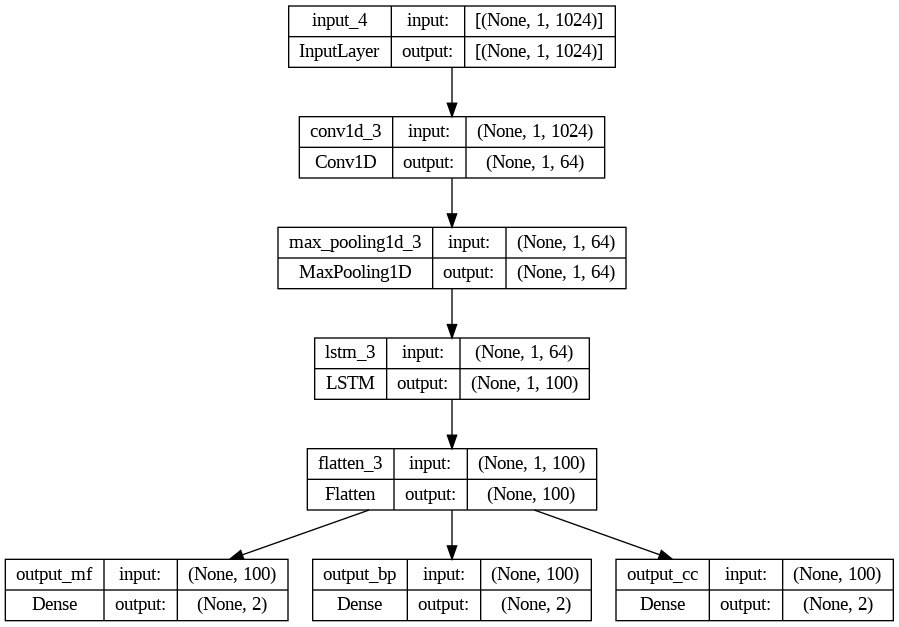
\includegraphics[scale=0.25]{img/model_diagram.png}
    \caption{Diagram of the Conv-LSTM model.}
    \label{fig:model_diagram}
\end{figure*}

\section{Results}

\subsection{Performance Evaluation}

\section{Discussion}

\section{Usage Overview}

\section{Code Availability}
The datasets used and all the code used for this project is available
at the following \href{https://github.com/marcouderzo/BioData-ProteinFunctionPrediction}{GitHub Repository}.



%-------------------------------------------------------------------------
\section{References}

List and number all bibliographical references in 9-point Times,
single-spaced, at the end of your paper. When referenced in the text,
enclose the citation number in square brackets, for
example.  Where appropriate, include the name(s) of
editors of referenced books.

%{\small
%\bibliographystyle{ieee_fullname}
%\bibliography{egbib}
%}

\end{document}
